\label{sec:results}

This section describes how the system was measured against the requirements
and specifications of section~4 of the approved Project Proposal, and then
gives every measurement that was taken, including those that fall short of a
target.

Three principles govern what follows. The first is that the \emph{classifier}
and the \emph{reproduction} are qualified on different material. Requirement
R2 asks the system to read and name real handwriting, so it is measured on
material held out from the network that performs the task. Requirement R1 asks
the system to reproduce text in a writer's style, so it is measured on pages the
robot itself drew; there the classifier is the measuring instrument and not the
subject, and it is admissible as an instrument only because qualification
test~2 establishes independently what it does on real handwriting.

The second principle is that a measurement is reported only against material
whose provenance was checked, not material assumed to be unseen. The reader and
the writer classifier were trained on different corpora, so what is held out
differs between them, and qualification test~2 establishes by transcript lookup
which lines are genuinely outside each network's training data before scoring
any of them. Where that check disqualified material, the material is excluded
and the exclusion is stated.

The third principle is that a line of handwriting is the unit of measurement.
Each page carries between three and eighteen lines, each line is scored
separately, and the number of lines behind every figure is stated.

Two machines were used, and which one produced a figure is stated with the
figure. The timing measurements of qualification tests~3 and~4 were taken on
the ODROID~N2+ that carries the deployed system, driving the real gantry, so
they describe the target platform. The accuracy measurements of qualification
tests~1, 2 and~6 were taken on the development computer, an x86-64 machine
running CPython~3.14; the platform affects how long those measurements took and
not what they were, because the same weights and the same arithmetic produce
the same answer on either machine. The geometry of qualification test~5 was
measured by hand off drawn paper and belongs to neither.

\subsection{Summary of results achieved} % REQUIRED HEADING
\label{sec:res-summary}

Table~\ref{tab:res-summary} compares the intended outcomes of the approved
Project Proposal with the outcomes that were measured. The first column
reproduces the requirement and its target specification as the proposal states
it, the second gives the measured value, and the third points to the
qualification test in which the measurement was made.

\begin{table}[h]
\centering
\fontsize{10}{12}\selectfont
\begin{tabularx}{\linewidth}{|>{\raggedright\arraybackslash}p{4.3cm}|>{\raggedright\arraybackslash}X|>{\raggedright\arraybackslash}p{2.2cm}|}
\hline
\textbf{Intended outcome} & \textbf{Actual outcome} & \textbf{Location in report} \\
\hline
\multicolumn{3}{|l|}{\textbf{Core mission requirements and specifications}} \\
\hline
R1: Reproduce text in the style of any writer of the training set, at least
85\,\% character accuracy and 85\,\% stylistic correlation. &
\textbf{Partially met.} Character accuracy over 184 drawn lines of 14 pages was
84.41\,\% (853 of 5\,471 characters wrong), 0.59 points below the target; word
accuracy was 45.97\,\%. The stylistic half was measured two ways and they
disagree. As the correlation the proposal specifies, it is \textbf{not met}:
the pooled coefficient over nine geometric features is 0.714 against a target
of 0.85. As writer identification from the robot's own output it is met: 159 of
184 lines, 86.4\,\% (95\,\% Wilson interval 80.7 to 90.6), and 14 of 14 pages
when a page's lines are pooled. &
Qualification test 1 \\
\hline
R2: Decode the text and identify the writer with an overall accuracy of at
least 95\,\%. &
\textbf{Partially met.} The writer was named correctly on 153 of 156 lines held
out from the writer classifier, 98.08\,\%, and on 11 of 11 writers when each
writer's lines are pooled, which exceeds the target. The text of 1\,076 lines
held out from the reader was read at 94.39\,\% character accuracy and 73.47\,\%
word accuracy, which is 0.61 points short of it. &
Qualification test 2 \\
\hline
R3: Reproduce text at no more than 4\,s per character. &
\textbf{Met.} Every complete reproduction recorded in the timing log met its
allowance. The worst case over all 26 recorded runs was 3.207\,s per character,
80.2\,\% of the allowance, on a 43-character block; over the nine attributable
runs of the 378-character paragraph the range was 1.343 to 2.705\,s per
character, at most 67.6\,\% of the allowance. &
Qualification test 3 \\
\hline
R4: Identify the writer and decode the text within $2+0.025x$\,s for $x$
characters. &
\textbf{Not met.} On the target platform a 500-character page took 46.26\,s
against an allowance of 14.50\,s and a 982-character page 55.49\,s against
26.55\,s. The two network stages exceed the per-character term of the allowance
by a factor of 1.6 to 2.4 and the four image stages exceed the fixed 2\,s term
by a factor of 8.1 to 8.4, so the requirement fails at every page length. &
Qualification test 4 \\
\hline
R5: Absolute gantry positional error of at most 0.5\,mm. &
\textbf{Met on the evidence available.} On a 100\,mm calibration square the
worst side was 0.30\,mm from nominal and the mean absolute error was 0.175\,mm.
One square and one triangle were measured, which is not sufficient for a
repeatability figure. &
Qualification test 5 \\
\hline
R6: At least 10 writing styles trained and stored permanently. &
\textbf{Met.} 11 writer styles are trained and stored: six from the public
database and five photographed for this project. &
Qualification test 6 \\
\hline
\multicolumn{3}{|l|}{\textbf{Field condition requirements and specifications}} \\
\hline
FC1: Operate on pages photographed by the system's own camera under ordinary
indoor lighting. &
\textbf{Met.} All 14 reproduction pages and all camera captures were
photographed indoors under room lighting with the system's own webcam at
$3264\times2448$, and were processed without manual adjustment. &
Qualification test 1, Qualification test 4 \\
\hline
FC2: Operate on ordinary unruled A4 paper with a ballpoint pen. &
\textbf{Met.} Every page reported here was drawn on unruled 80\,g/m\textsuperscript{2}
A4 with the same ballpoint pen in the gantry pen holder. &
Qualification test 1 \\
\hline
\end{tabularx}
\caption{Summary of results achieved.}
\label{tab:res-summary}
\end{table}

\subsection{Qualification tests} % REQUIRED HEADING
\label{sec:res-qtp}

The tests below appear in the order of importance of the requirements in
section~4 of the approved Project Proposal. Each test states its objective, the
equipment and the software written to perform it, the parameters and steps, the
measurements, the observations that follow from them without interpretation,
and, where the sample supports one, a statistical analysis.

\subsubsection{Test material and the software written to perform the tests}
\label{sec:res-material}

One body of test material serves the first two tests and is described once
here. Fourteen pages were drawn by the robot, one or two for each of eleven
writers, and each page carries up to three blocks of text chosen to separate
three different questions. Block~A is a 378-character paragraph, long enough to
occupy eight to seventeen written lines, which exercises line segmentation and
general text accuracy together. Block~B is the 43-character pangram ``The quick
brown fox jumps over the lazy dog'', which contains every letter of the
alphabet and occupies one or two lines, so it tests reading and writer
identification on a single line with no multi-line segmentation to confound
them. Block~C is a passage taken from the writer's own source material, which is
the only text of the three that the writer themselves actually wrote.

Each drawn page was photographed, segmented into line crops, and every crop was
read and classified separately, giving 184 line samples in total. A transcript
was prepared for every page with one line of text for each written line, so
that a read line and its intended text can be compared one to one; the line
breaks of each transcript were taken from that page's own segmentation overlay
and not assumed.

\paragraph{Software written for the tests.}
Five programs were written for this chapter and no part of the measurement is
done by hand.
\texttt{blocks\_master.py} segments each drawn page, reads and classifies every
line, assigns each line to its block, and writes one record per line;
\texttt{holdout\_text.py} and the writer half of the same harness score the
held-out real crops;
\texttt{cursivity.py} measures how joined each writer's genuine hand is;
\texttt{style\_distance.py} places the writers in a style space and measures
how far each is from the others;
\texttt{classify\_gcode.py} renders a G-code job to an image and classifies it
without the page ever being drawn.
All figures in this chapter are produced by \texttt{make\_results\_figures.py}
from a single colour and font definition, so that every figure is formatted
alike.

\medskip
    \QualificationTest{Reproduction of text in a writer's style (R1)}

        \medskip
        \QualificationSection{Objectives of the test or experiment}

        To determine whether text drawn by the robot in a stored writer's style
        is legible as the intended text, and whether it still carries the
        identity of that writer. R1 sets two targets, 85\,\% character accuracy
        and 85\,\% stylistic correlation, and both are measured here.

        \medskip
        \QualificationSection{Equipment used}

        The gantry described in Section~\ref{sec:gantry}, driven by an
        ODROID~N2+; a Logitech C270 webcam at $3264\times2448$ mounted above the
        platen; unruled 80\,g/m\textsuperscript{2} A4 paper; a 0.7\,mm ballpoint
        pen in the gantry pen holder; and a 150\,mm vernier caliper reading to
        0.01\,mm for the page measurements. Scoring used the software named in
        Section~\ref{sec:res-material}.

        \medskip
        \QualificationSection{Test setup and experimental parameters}

        Pages were drawn at a pen-down feed of 800\,mm/min and a pen-up feed of
        4\,000\,mm/min, with the best-of-$N$ synthesis search at $N=1$ except
        for the two most joined hands. The writer was identified by the
        stroke-normalised shape classifier
        \texttt{author\_shape\_11\_pw170\_weights.npz}, which redraws every crop
        at a constant pen width of 0.17 x-heights before classifying it, and the
        text was read by \texttt{paper\_cnn\_bilstm\_ctc\_joint\_best.npz} with
        greedy decoding, no beam search, no language model and no lexicon.
        Writers 151 and 551 were withdrawn from the trained set, so the
        classifier chooses between 11 writers and chance is 9.1\,\%.

        \medskip
        \QualificationSection{Steps followed in the test or experiment}

        \begin{enumerate}
        \item Synthesise each block of text in the stored style of the writer
              and emit G-code.
        \item Draw the page on the gantry and photograph it with the system's
              own camera.
        \item Segment the photograph into line crops and confirm that the number
              of crops equals the number of transcript lines.
        \item Read every crop and score it against its transcript line.
        \item Classify every crop and record the writer named, the confidence,
              and the probability given to the true writer.
        \item Pool the lines of a page by ink to obtain one writer per page.
        \end{enumerate}

        \medskip
        \QualificationSection{Results or measurements}

        Table~\ref{tab:res-r1-blocks} gives the result by block and
        Table~\ref{tab:res-r1-writer} by writer. Character and word accuracy are
        reported as micro averages, that is one sum of edit distances over one
        sum of reference characters, so that a long line counts for more than a
        short one; the macro average over all 184 lines, which weighs every line
        alike, is 82.04\,\% character and 48.80\,\% word.
        Figure~\ref{fig:res-blocks} shows the same block figures with their
        intervals, Figure~\ref{fig:res-per-author} the per-writer figures, and
        Figure~\ref{fig:res-confusion-rep} the full confusion of writer
        identification over the 184 lines.

\begin{table}[h]
\centering
\fontsize{10}{12}\selectfont
\begin{tabular}{|l|r|r|r|r|}
\hline
\textbf{Block} & \textbf{Lines} & \textbf{Writer identified} & \textbf{Character} & \textbf{Word} \\
\hline
A: paragraph, many lines      & 119 & 91.6\,\% [85.2, 95.4] & 84.88\,\% & 47.87\,\% \\
B: pangram, single line       &  21 & 76.2\,\% [54.9, 89.4] & 78.40\,\% & 41.41\,\% \\
C: writer's own source text   &  44 & 77.3\,\% [63.0, 87.2] & 85.32\,\% & 40.91\,\% \\
\hline
All three blocks              & 184 & 86.4\,\% [80.7, 90.6] & 84.41\,\% & 45.97\,\% \\
\hline
\end{tabular}
\caption{Reproduction accuracy by block of text, over the 14 drawn pages.
Bracketed figures are 95\,\% Wilson intervals on the proportion of lines whose
writer was identified correctly. Character and word accuracy are micro
averages.}
\label{tab:res-r1-blocks}
\end{table}

\begin{table}[h]
\centering
\fontsize{10}{12}\selectfont
\begin{tabular}{|l|r|r|r|r|r|}
\hline
\textbf{Writer} & \textbf{Lines} & \textbf{Writer identified} & \textbf{Character} & \textbf{Word} & \textbf{Comp./char} \\
\hline
Y   & 13 & 92.3\,\% [66.7, 98.6]  & 97.01\,\% & 74.16\,\% & 0.739 \\
150 & 13 & 53.8\,\% [29.1, 76.8]  & 96.75\,\% & 76.40\,\% & 0.766 \\
O   & 16 & 100.0\,\% [80.6, 100]  & 94.25\,\% & 58.51\,\% & 0.951 \\
B   & 16 & 93.8\,\% [71.7, 98.9]  & 93.11\,\% & 68.24\,\% & 0.980 \\
384 & 16 & 87.5\,\% [64.0, 96.5]  & 86.93\,\% & 43.18\,\% & 0.681 \\
552 & 15 & 80.0\,\% [54.8, 93.0]  & 86.17\,\% & 48.39\,\% & 0.609 \\
152 & 15 & 80.0\,\% [54.8, 93.0]  & 85.74\,\% & 49.44\,\% & 0.512 \\
A   & 27 & 100.0\,\% [87.5, 100]  & 77.29\,\% & 18.09\,\% & 0.527 \\
153 & 19 & 57.9\,\% [36.3, 76.9]  & 75.72\,\% & 31.46\,\% & 0.255 \\
588 & 18 & 94.4\,\% [74.2, 99.0]  & 73.19\,\% & 22.99\,\% & 0.547 \\
T   & 16 & 100.0\,\% [80.6, 100]  & 60.97\,\% & 13.41\,\% & 0.208 \\
\hline
\end{tabular}
\caption{Reproduction accuracy by writer, ordered by character accuracy.
A, B, O, T and Y are the five photographed contributors; the numbered writers
are from the public database. The last column is connectedness, measured as
connected ink components per character on the writer's own genuine pages, where
a lower value is a more joined hand.}
\label{tab:res-r1-writer}
\end{table}

\begin{figure}[h]
\centering
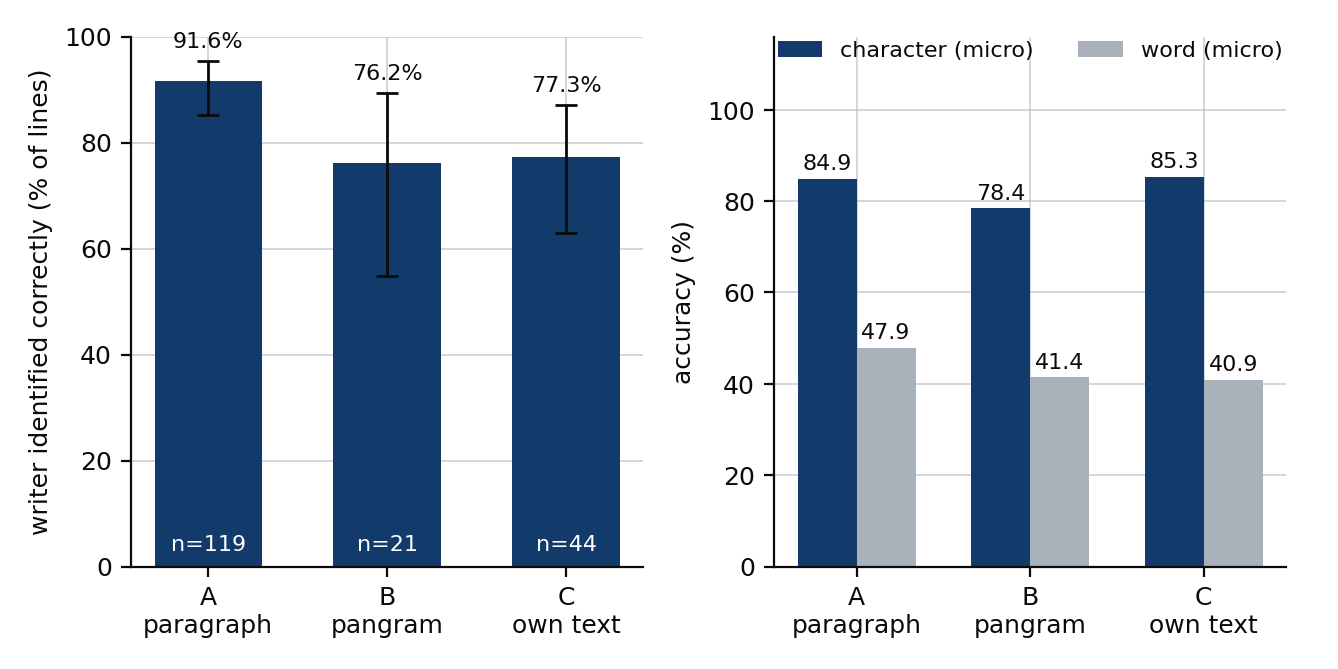
\includegraphics[width=0.95\linewidth]{Figures/res_blocks.png}
\caption{Reproduction accuracy by block. The left panel is the proportion of
lines whose writer was identified correctly, with 95\,\% Wilson intervals and
the number of lines behind each bar; the right panel is micro-averaged
character and word accuracy.}
\label{fig:res-blocks}
\end{figure}

\begin{figure}[h]
\centering
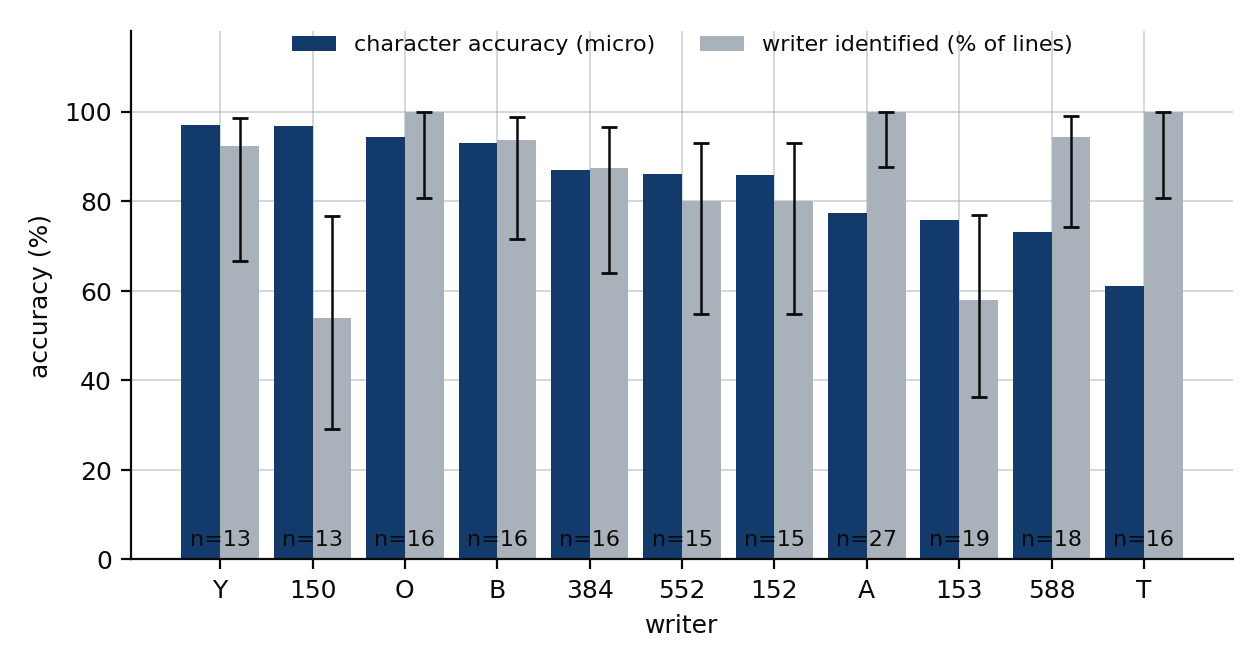
\includegraphics[width=0.95\linewidth]{Figures/res_per_author.png}
\caption{Reproduction accuracy by writer, ordered by character accuracy. Dark
bars are micro-averaged character accuracy and silver bars the proportion of
lines whose writer was identified, with 95\,\% Wilson intervals.}
\label{fig:res-per-author}
\end{figure}

\begin{figure}[h]
\centering
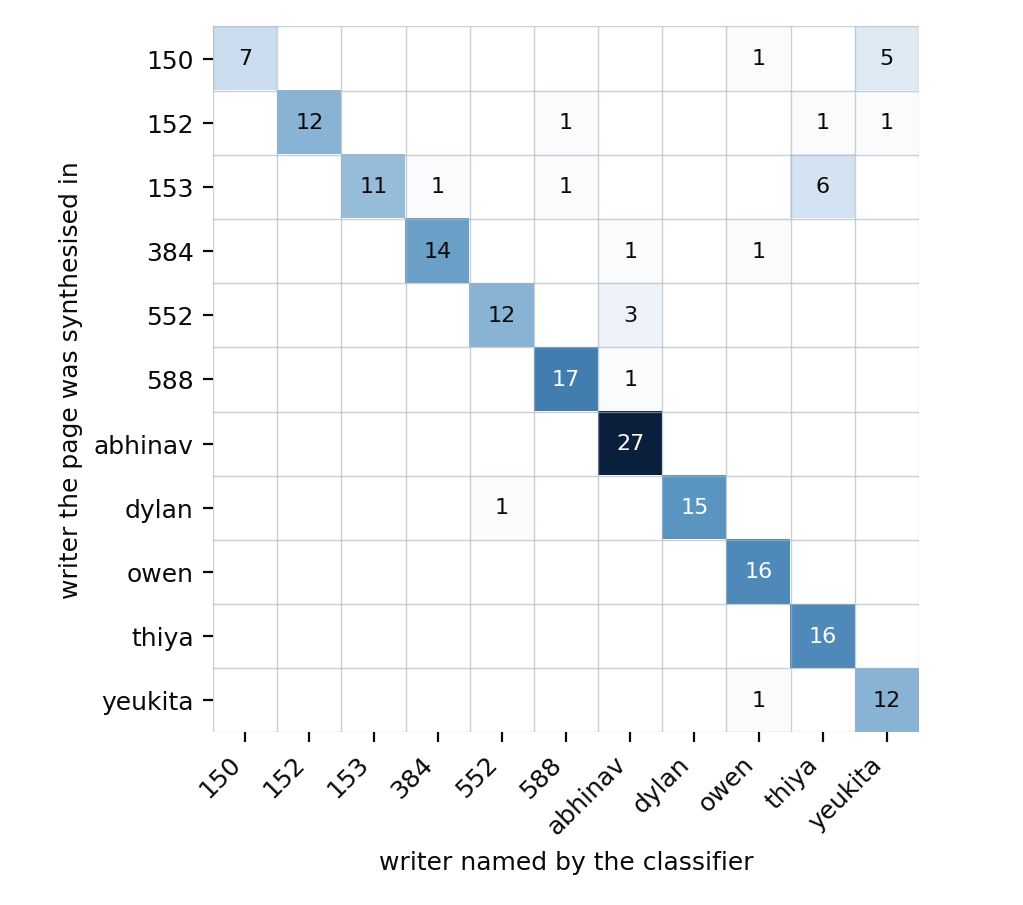
\includegraphics[width=0.85\linewidth]{Figures/res_confusion_reproduced.png}
\caption{Writer identification over the 184 drawn lines. Rows are the writer the
page was synthesised in and columns the writer the classifier named; the
diagonal holds the 159 correct lines. Empty cells are zero.}
\label{fig:res-confusion-rep}
\end{figure}

        Connectedness was measured on each writer's genuine pages as the number
        of connected ink components per character, over 45 sampled real line
        crops per writer. Against character accuracy the Pearson coefficient is
        $r=+0.855$ and the Spearman rank coefficient $\rho=+0.845$ over the 11
        writers; against word accuracy $r=+0.771$ and $\rho=+0.782$; against the
        proportion of lines whose writer was identified, $r=+0.170$ and
        $\rho=-0.027$. Figure~\ref{fig:res-connectedness} plots the first and
        the last of these.

\begin{figure}[h]
\centering
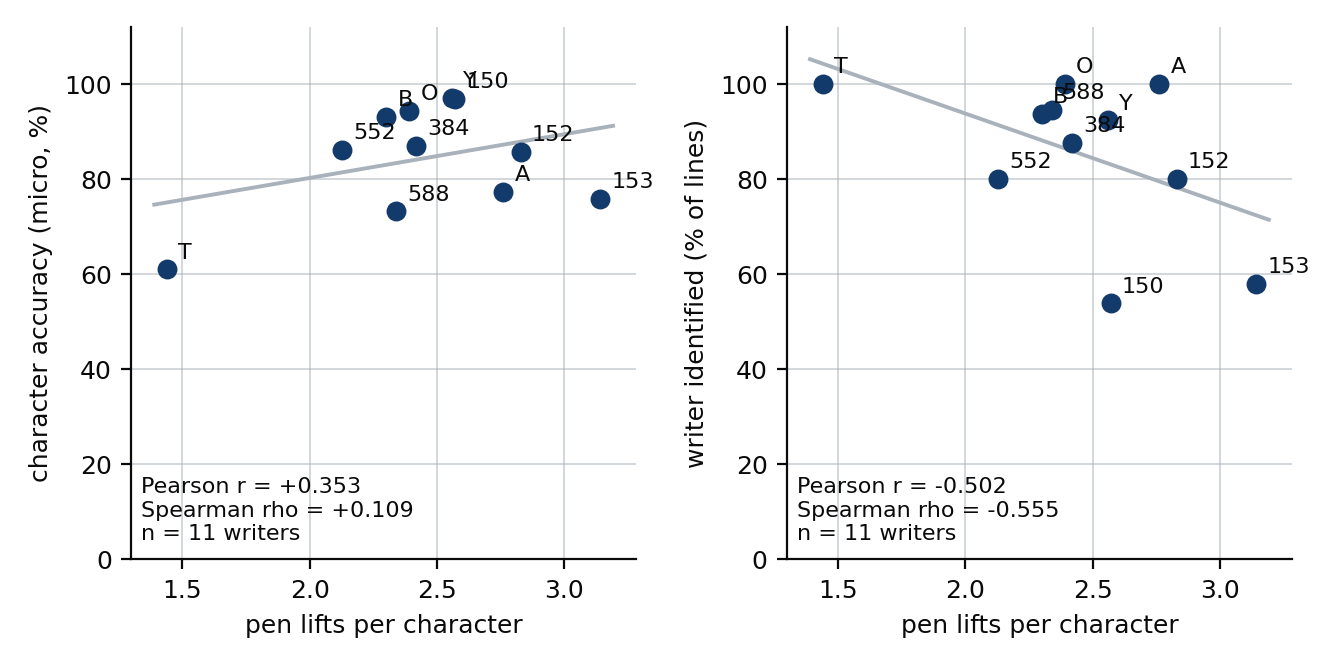
\includegraphics[width=0.95\linewidth]{Figures/res_connectedness.png}
\caption{Accuracy against connectedness. The horizontal axis is connected ink
components per character on the writer's own handwriting, where a lower value is
a more joined hand. The grey line is a least-squares fit and the coefficients
are printed on each panel.}
\label{fig:res-connectedness}
\end{figure}

        A writer may also be hard to identify because another writer's hand
        resembles theirs. To measure this, each writer was placed in a style
        space of eight standardised geometric descriptors taken from their own
        style profile --- slant, x-height, ascender and descender extent, stroke
        width, ink fraction, aspect ratio and mid-band fraction --- and the
        Euclidean distance to the nearest other writer was computed. Against the
        proportion of lines whose writer was identified, that distance gives
        $r=-0.244$ and $\rho=-0.100$. The three largest confusions of
        Figure~\ref{fig:res-confusion-rep} are 153 named as T on 6 lines, 150
        named as Y on 5 lines and 552 named as A on 3 lines; in none of the
        three is the named writer the true writer's nearest neighbour in that
        style space, which are A, 152 and 588 respectively.

        Six G-code jobs were rendered to images and classified without being
        drawn, which separates what the synthesis produces from what the gantry
        then does with it. Table~\ref{tab:res-gcode} gives the result.

\begin{table}[h]
\centering
\fontsize{10}{12}\selectfont
\begin{tabular}{|l|r|r|l|r|r|}
\hline
\textbf{G-code job} & \textbf{Lines} & \textbf{Text lines} & \textbf{Named} & \textbf{Conf.} & \textbf{Lines agreeing} \\
\hline
\texttt{2b7e03f1} & 9\,399  &  8 & O & 86.0\,\% & 7/8 \\
\texttt{99f136a0} & 5\,889  &  7 & O & 66.7\,\% & 6/7 \\
\texttt{bc8d7860} & 13\,747 & 17 & A & 75.6\,\% & 15/17 \\
\texttt{a6393598} & 9\,766  & 11 & B & 29.3\,\% & 4/11 \\
\texttt{16d4c05b} & 1\,255  &  2 & B & 72.4\,\% & 2/2 \\
\texttt{bfa7a5dc} & 1\,288  &  1 & Y & 79.2\,\% & 1/1 \\
\hline
\end{tabular}
\caption{Writer identification from the G-code alone, with no page drawn. The
job \texttt{2b7e03f1} has 9\,399 G-code lines, which is the count the server log
records for the run annotated \texttt{Owen\_curated}.}
\label{tab:res-gcode}
\end{table}

        R1's stylistic specification is stated as a correlation, and it was
        measured as one. Nine geometric features were extracted from each
        writer's genuine lines and from the system's reproduction of the same
        text, and the Pearson coefficient between the two was taken feature by
        feature and pooled. A separate overlay test measured how far a
        reproduction sits from the hand it imitates against how far it sits from
        the other writers' hands, reduced to the ratio of the two mean distances
        and the area under the resulting curve.
        Table~\ref{tab:res-r1-style} gives both;
        Table~\ref{tab:res-perfeature} in the appendix gives the nine features
        separately and Figure~\ref{fig:res-dist} the two distance distributions.

\begin{table}[h]
\centering
\fontsize{10}{12}\selectfont
\begin{tabular}{|l|r|r|l|}
\hline
\textbf{Measure} & \textbf{Measured} & \textbf{Target} & \textbf{Verdict} \\
\hline
Pooled style correlation over nine features & 0.714 & 0.85 & Not met \\
Best single feature (slant)                 & 0.996 & --- & --- \\
Worst single feature (descender extent)     & 0.148 & --- & --- \\
\hline
Overlay distance ratio, mismatched to matched & 2.2 & --- & --- \\
Overlay area under the curve                  & 0.71 & --- & --- \\
\hline
Writer identified from the drawn output, by line & 86.4\,\% & 85\,\% & Met \\
Writer identified from the drawn output, by page & 14/14 & --- & Met \\
\hline
\end{tabular}
\caption{The two ways R1's stylistic half was measured. The correlation is the
measure the proposal states and it falls 0.136 below its target; writer
identification from the machine's own output exceeds 85\,\%. An area under the
curve of 0.5 would mean the reproduction carries no writer information at all.}
\label{tab:res-r1-style}
\end{table}

        A third measurement of style was taken that involves no classifier at
        all. The same 378-character paragraph was prepared for every one of the
        eleven writers, and the geometry of the resulting G-code was measured
        directly: the pen-down path length, which is the quantity of ink the
        machine would lay down, and the number of pen lifts, which is how often
        the hand leaves the paper. Both are properties of the emitted tool path
        and are read off it arithmetically, so neither can be influenced by the
        network that selects candidates. Figure~\ref{fig:res-style-signature}
        gives both for identical text.

\begin{figure}[h]
\centering
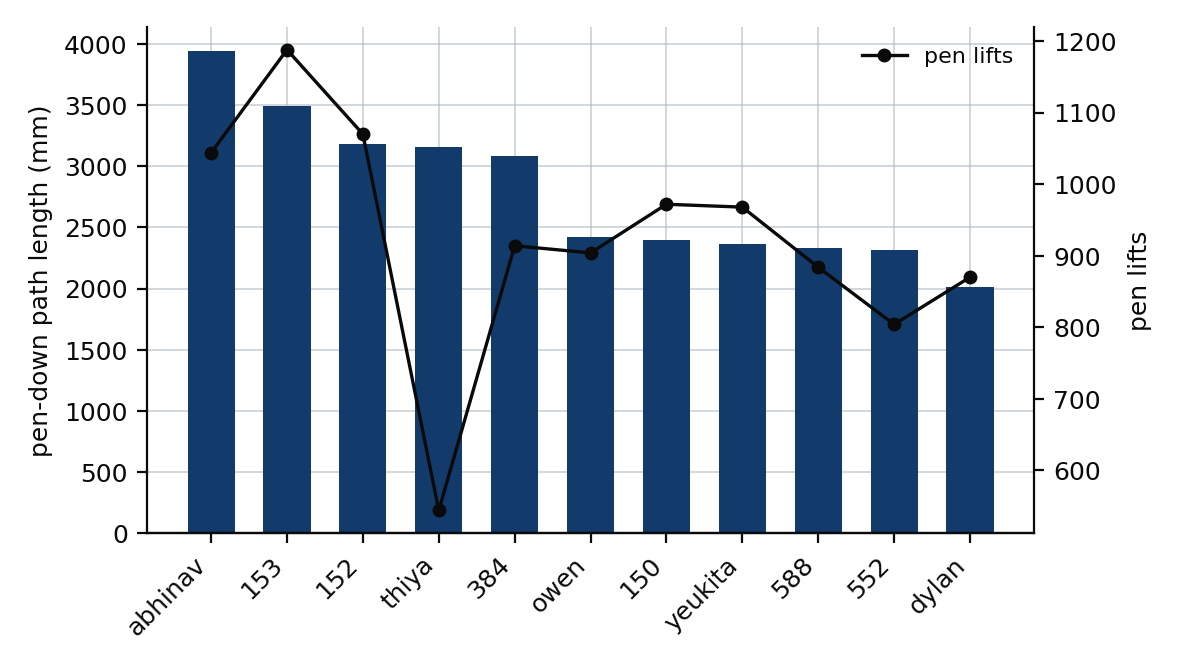
\includegraphics[width=0.92\linewidth]{Figures/res_style_signature.png}
\caption{Pen-down path length and pen lifts for the same 378-character
paragraph prepared in each of the eleven writers' styles, measured from the
G-code before any page was drawn. Bars are the path length against the left
axis and the line is the pen-lift count against the right axis; writers are
ordered by path length.}
\label{fig:res-style-signature}
\end{figure}

        \medskip
        \QualificationSection{Observations}

        Character accuracy over all 184 lines is 84.41\,\%, which is 0.59 points
        below the 85\,\% target; 853 of 5\,471 characters were wrong. The
        proportion of lines whose writer was identified is 86.4\,\%, above the
        85\,\% figure, and all 14 pages were attributed to the correct writer
        when their lines were pooled.

        Of the three blocks, block~A has the highest proportion of lines
        identified at 91.6\,\% and block~B the lowest at 76.2\,\%. Block~C has
        the highest character accuracy at 85.32\,\% and block~B the lowest at
        78.40\,\%. The intervals of blocks~B and~C overlap over most of their
        range.

        Character accuracy by writer spans 60.97\,\% to 97.01\,\%, a range of
        36.0 points. Four writers exceed 93\,\%: Y, 150, O and B. The four are
        also the four least joined hands of the eleven, with 0.739 to 0.980
        components per character. The three lowest character accuracies are T,
        588 and 153, and two of those three, T at 0.208 and 153 at 0.255, are the
        two most joined hands measured.

        The rank correlation between connectedness and character accuracy is
        $\rho=+0.845$; between connectedness and the proportion of lines
        identified it is $\rho=-0.027$. The rank correlation between distance to
        the nearest writer in style space and the proportion of lines identified
        is $\rho=-0.100$.

        Three writers were identified on every line: A, O and T. Two writers
        were identified on fewer than 60\,\% of their lines: 150 at 53.8\,\% and
        153 at 57.9\,\%. The writer with the highest character accuracy, Y at
        97.01\,\%, and the writer with the lowest, T at 60.97\,\%, were
        identified on 92.3\,\% and 100\,\% of their lines respectively.

        Of the six G-code jobs classified before drawing, five were named with
        between 66.7\,\% and 86.0\,\% confidence and agreement on at least six of
        every seven lines; one, \texttt{a6393598}, was named at 29.3\,\% with
        four of eleven lines agreeing.

        For the same 378-character paragraph prepared in all eleven styles, the
        pen-down path length ranges from 2\,015.4\,mm to 3\,942.8\,mm, a factor
        of 1.96, and the pen-lift count from 544 to 1\,188, a factor of 2.18.
        The two do not rank together: the writer with the fewest pen lifts, T at
        544, has the fourth longest path at 3\,157.7\,mm, and the writer with
        the most lifts, 153 at 1\,188, has the second longest at 3\,494.4\,mm.

        \medskip
        \QualificationSection{Statistical analysis}

        The 95\,\% intervals in Tables~\ref{tab:res-r1-blocks}
        and~\ref{tab:res-r1-writer} are Wilson score intervals, which are used
        in place of the normal approximation because several cells hold fewer
        than 20 lines and the normal interval would extend past 100\,\%. The
        interval on the pooled 184 lines is 80.7 to 90.6\,\%, so the lower bound
        lies below the 85\,\% figure and the result is not separated from the
        target by this sample.

        The correlations are reported with both the Pearson and the Spearman
        coefficient because $n=11$ and a single writer can move a Pearson
        coefficient appreciably. For character accuracy against connectedness
        the two agree closely, $+0.855$ and $+0.845$; for writer identification
        against connectedness they do not, $+0.170$ and $-0.027$.

        No correction for multiple comparisons has been applied to the five
        correlations reported, and at $n=11$ writers none of them is separated
        from zero with the confidence that a larger sample would allow.

\medskip
    \QualificationTest{Reading the text and naming the writer of unseen
    handwriting (R2)}

        \medskip
        \QualificationSection{Objectives of the test or experiment}

        To determine the accuracy with which the system reads the text of, and
        names the writer of, handwriting that the network performing the task
        was not trained on. R2 sets a single target of 95\,\% overall accuracy.
        The two halves are performed by two separate networks trained on
        different corpora, so each is measured on material held out from that
        network, and the two halves are reported separately.

        \medskip
        \QualificationSection{Equipment used}

        No gantry hardware is involved. The development computer described at
        the head of this section was used, with two trained networks: the
        reader, checkpoint \texttt{paper\_cnn\_bilstm\_ctc\_scratch\_best.npz},
        and the writer classifier, checkpoint
        \texttt{author\_shape\_11\_pw170\_weights.npz}, which was trained on
        crops redrawn at a constant pen width of 0.17 x-heights. Two scoring
        programs were written for this test: one that scores the reader against
        a transcript line by line, and one that indexes the public corpus by
        transcript so that the provenance of every line can be established.

        \medskip
        \QualificationSection{Test setup and experimental parameters}

        The two networks have different training corpora, so the held-out
        material differs between the two halves of the test, and establishing
        what is genuinely held out is part of the test.

        \emph{The reader.} The reader was trained on the IAM line corpus as
        distributed by Teklia, mixed with the photographed writers' lines. That
        corpus arrives already partitioned into a \texttt{train} directory of
        6\,481 line crops and a \texttt{validation} directory of 976. The
        training loop reads the first through the optimiser and the second only
        through the evaluation path, so no weight is ever updated from the
        validation crops. Those 976 crops are therefore held out by
        construction, and because they are the corpus's own line cuts they also
        carry no dependence on this project's segmenter. The photographed
        writers contribute a further 100 held-out lines, a seeded 15\,\% of
        their lines fixed by the recorded split seed. The text half is measured
        on these 1\,076 lines.

        The database writers' own pages are \emph{not} used for the text half,
        and the reason is a provenance check rather than a preference. Every
        labelled line of those pages was looked up in the public corpus by
        normalised transcript. For writer~150, 84 of its 91 labelled lines were
        found in the \texttt{train} directory; for writer~152, 80 of 87; for
        writer~153, 83 of 97. Those lines are in the reader's training data and
        cannot measure it. The remaining database writers' pages were found in
        neither directory, so they lie outside the corpus the reader was trained
        on rather than being held out from it, and they are excluded for that
        reason. Not one line of any database writer appears in the
        \texttt{validation} directory, so the two held-out sets used below share
        no line with each other.

        \emph{The writer classifier.} The classifier was trained only on the
        eleven writers' own pages and never on the public corpus, so its
        held-out material is the project's own split, fixed by seed: the last
        labelled page of each database writer, and the seeded 15\,\% of each
        photographed writer's lines. That gives 156 held-out lines, 56 from
        database writers and 100 from photographed writers. The public
        corpus cannot contribute to this half, because its crops are
        distributed without a writer identity.

        \medskip
        \QualificationSection{Steps followed in the test or experiment}

        \begin{enumerate}
        \item Index every transcript in both directories of the public corpus,
              and look up each database writer's labelled lines to establish
              which are in the reader's training data.
        \item Read all 976 held-out crops of the public corpus with the reader
              and score each against its transcript.
        \item Rebuild the photographed writers' data set, apply the project's
              seeded split, and read the 100 held-out lines in the same way.
        \item Redraw each of the 156 crops held out from the writer classifier
              at a constant pen width of 0.17 x-heights, classify it, and
              compare the named writer with the label.
        \item Pool the lines of each held-out page by ink to obtain one writer
              per page.
        \end{enumerate}

        \medskip
        \QualificationSection{Results or measurements}

        Table~\ref{tab:res-r2-text} gives the text half over the 1\,076 lines
        held out from the reader, Table~\ref{tab:res-r2-writer} the writer half
        over the 156 lines held out from the classifier, and
        Figure~\ref{fig:res-confusion-hold} the confusion of writer
        identification over those same 156 lines.

\begin{table}[h]
\centering
\fontsize{10}{12}\selectfont
\begin{tabular}{|l|r|r|r|r|r|}
\hline
\textbf{Held-out set} & \textbf{Lines} & \textbf{Characters} & \textbf{Character} & \textbf{Word} & \textbf{Lines exact} \\
\hline
Public corpus, validation split & 976 & 42\,072 & 94.39\,\% & 73.67\,\% & 212 \\
\hline
Photographed writer A &  31 &   934 & 94.65\,\% & 76.92\,\% &  9 \\
Photographed writer B &  19 &   739 & 97.70\,\% & 84.73\,\% &  9 \\
Photographed writer O &  22 & 1\,017 & 94.79\,\% & 69.05\,\% &  8 \\
Photographed writer T &  11 &   345 & 89.28\,\% & 57.69\,\% &  1 \\
Photographed writer Y &  17 &   640 & 92.50\,\% & 54.62\,\% &  3 \\
\hline
All photographed writers & 100 & 3\,675 & 94.42\,\% & 70.74\,\% & 30 \\
\hline
\textbf{All held-out lines} & \textbf{1\,076} & \textbf{45\,747} & \textbf{94.39\,\%} & \textbf{73.47\,\%} & \textbf{242} \\
\hline
\end{tabular}
\caption{Reading 1\,076 lines of handwriting held out from the reader.
Character and word accuracy are micro averages over the character and word
counts shown. The validation split is the public corpus's own held-out
partition; the photographed writers' lines are a seeded 15\,\% of their own.
``Lines exact'' counts lines read with no error at all.}
\label{tab:res-r2-text}
\end{table}

\begin{table}[h]
\centering
\fontsize{10}{12}\selectfont
\begin{tabular}{|l|r|r|r|}
\hline
\textbf{Writer} & \textbf{Held-out lines} & \textbf{Lines named correctly} & \textbf{Page named correctly} \\
\hline
150 &   9 &   8/9 & Yes \\
152 &   8 &   7/8 & Yes \\
153 &   9 &   9/9 & Yes \\
384 &  12 & 12/12 & Yes \\
552 &  10 & 10/10 & Yes \\
588 &   8 &   8/8 & Yes \\
A   &  31 & 31/31 & Yes \\
B   &  19 & 18/19 & Yes \\
O   &  22 & 22/22 & Yes \\
T   &  11 & 11/11 & Yes \\
Y   &  17 & 17/17 & Yes \\
\hline
\textbf{All} & \textbf{156} & \textbf{153/156 = 98.08\,\%} & \textbf{11/11} \\
\hline
\end{tabular}
\caption{Naming the writer of 156 lines held out from the writer classifier.
The database writers' held-out material is the last labelled page of each
writer and the photographed writers' a seeded 15\,\% of their lines. The last
column pools the lines of each writer's held-out material by ink and names one
writer from the pool.}
\label{tab:res-r2-writer}
\end{table}

\begin{figure}[h]
\centering
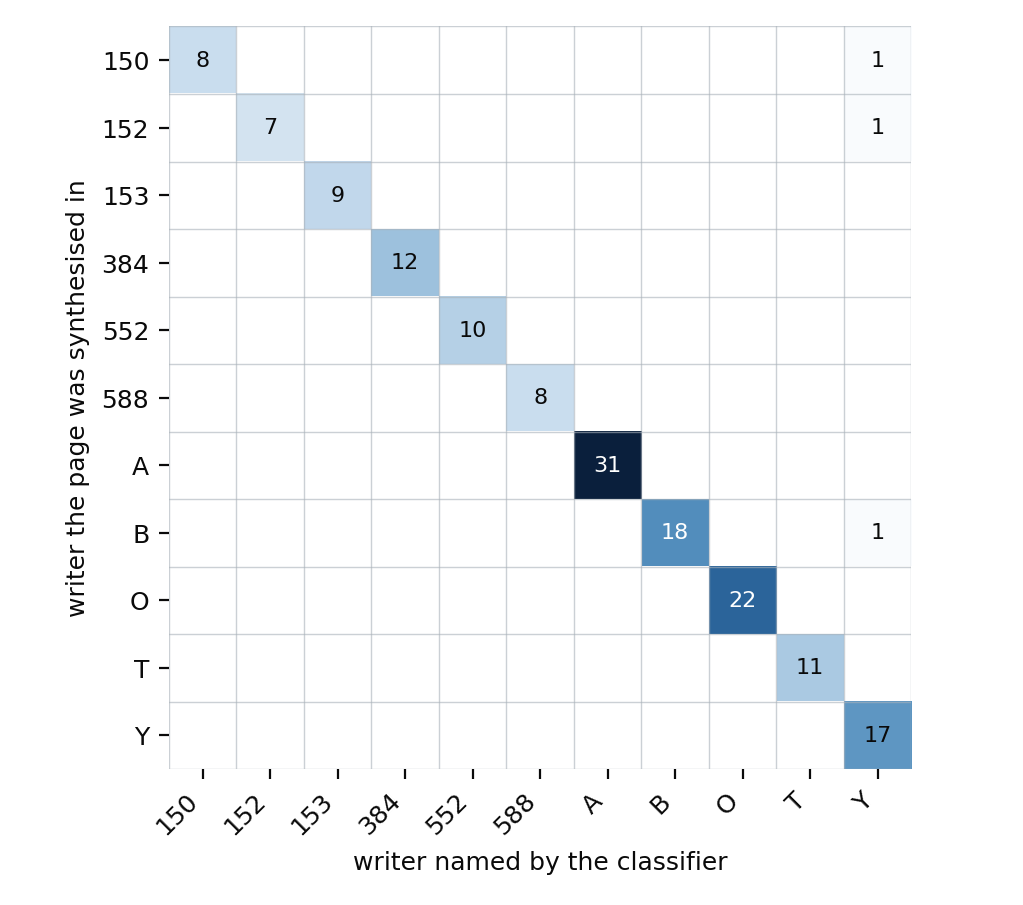
\includegraphics[width=0.85\linewidth]{Figures/res_confusion_holdout.png}
\caption{Writer identification over the 156 lines held out from the writer
classifier. Rows are the true writer and columns the writer named; three lines
are off the diagonal. Empty cells are zero.}
\label{fig:res-confusion-hold}
\end{figure}

        \medskip
        \QualificationSection{Observations}

        The writer was named correctly on 153 of 156 held-out lines, 98.08\,\%,
        which is 3.08 points above the 95\,\% target. Pooling each writer's
        held-out lines by ink names all 11 writers correctly.

        The three errors fall on three different writers, one line each, and all
        three were named as the same writer, Y. All three are the last line of
        the writer's held-out material: line 9 of 9 for writer~150, line 8 of 8
        for writer~152 and line 19 of 19 for writer~B. Eleven of the 156 lines
        are last lines.

        The three incorrect lines were named at 44.2\,\%, 83.8\,\% and 39.5\,\%
        confidence. Over the 153 correct lines the median confidence is 99.9\,\%
        and the mean 97.7\,\%; over the three incorrect lines the mean is
        55.8\,\%. Six lines in total were named at below 80\,\% confidence, of
        which two are among the three errors.

        The text of the 1\,076 lines held out from the reader was read at
        94.39\,\% character accuracy, 2\,565 of 45\,747 characters wrong, and
        73.47\,\% word accuracy. This is 0.61 points below the 95\,\% target on
        characters and 21.53 points below it on words. Of the 1\,076 lines, 242
        were read with no error at all.

        The two held-out sets agree closely with each other. The public
        corpus's 976 crops were read at 94.39\,\% and the 100 photographed lines
        at 94.42\,\%, a difference of 0.03 points. Word accuracy differs more,
        73.67\,\% against 70.74\,\%.

        Character accuracy by photographed writer spans 89.28\,\% to 97.70\,\%,
        a range of 8.4 points. The proportion of lines read with no error at all
        spans 9.1\,\% to 47.4\,\% over the same five writers, against 21.7\,\%
        on the public corpus.

        \medskip
        \QualificationSection{Statistical analysis}

        The 95\,\% Wilson score interval on 153 of 156 lines named correctly is
        94.5 to 99.3\,\%. The lower bound lies 0.5 points below the 95\,\%
        target, so this sample places the result above the target as a point
        estimate but does not separate it from the target at 95\,\% confidence.
        Pooling by writer gives 11 of 11, whose interval is 74.1 to 100\,\%; a
        count of eleven cannot resolve a 95\,\% target, which is why the
        per-line figure is the one quoted.

        A worst-case bound can be placed on the same sample without assuming
        that any low-confidence line is right. Taking every line named at below
        80\,\% confidence to be wrong, whether it was or not, leaves 149 of 156
        correct, 95.51\,\%, which is still above the 95\,\% target. The result
        therefore clears the target on the pessimistic reading as well as on the
        measured one.

        The concentration of the three errors on last lines was tested against
        chance. Eleven of the 156 lines are last lines, so under the hypothesis
        that errors fall uniformly the probability that all three land on one is
        $(11/156)^{3}=3.5\times10^{-4}$. The pattern is therefore unlikely to be
        an accident of this sample, although three events cannot establish its
        cause.

        No interval is quoted on the text half, because character accuracy is a
        ratio of edit distance to character count and not a count of successes,
        so a binomial interval does not apply to it. The proportion of lines
        read with no error at all is a count and can carry one: 242 of 1\,076 is
        22.5\,\%, with an interval of 20.1 to 25.1\,\%.

        The two halves are measured on different material by different networks
        and are independent of one another. Within the text half the 976 public
        crops and the 100 photographed lines are disjoint, which was established
        by the transcript lookup described above, so the pooled figure does not
        double-count any line. The public corpus contributes 92.0\,\% of the
        characters in the pooled figure, so the pooled value is close to the
        public-corpus value by construction, and the photographed writers'
        figure is reported separately for that reason.

\medskip
    \QualificationTest{Time taken to reproduce text (R3)}

        \medskip
        \QualificationSection{Objectives of the test or experiment}

        To determine whether a page is drawn within the allowance of 4\,s per
        character set by R3.

        \medskip
        \QualificationSection{Equipment used}

        The gantry and the ODROID~N2+ as in qualification test~1. Timing was
        taken by the server's own instrumentation, which records the synthesis,
        rendering, G-code and drawing stages separately, and was read from the
        server console log.

        \medskip
        \QualificationSection{Test setup and experimental parameters}

        Runs were made at a pen-down feed of 800\,mm/min and a pen-up feed of
        4\,000\,mm/min. A reproduction is asked for in two requests, one that
        generates the page and one that draws it, and the drawing request
        carries the generation stages forward into its own total, so a timing
        block that contains a drawing stage is the \emph{complete} reproduction
        and a generation-only block is a part of one. Only blocks containing a
        drawing stage are counted here, which prevents the synthesis time from
        being counted twice.

        Three exclusions are applied and are stated so that they are visible.
        The log is written in two layouts, one to the server console and one to
        the browser panel, and a run that appears in both is counted once: 47
        blocks with a drawing stage reduce to 43 distinct runs. Seven of those
        were stopped before the page was finished, which is detectable because
        their drawing stage falls below 1\,s per character against a going rate
        of 2 to 3\,s per character, and they are set aside as incomplete. That
        leaves 36 complete reproductions, spanning nine block lengths from 43 to
        378 characters.

        \medskip
        \QualificationSection{Steps followed in the test or experiment}

        \begin{enumerate}
        \item Submit a block of text and a writer to the server and record the
              character count.
        \item Draw the page, with the server recording each stage separately.
        \item Read the total and the per-stage times from the log.
        \item Discard duplicate layouts of the same run and blocks whose drawing
              stage shows the job was stopped early.
        \item Compare each total against the allowance of 4\,s per character,
              and record the worst case at each block length.
        \end{enumerate}

        \medskip
        \QualificationSection{Results or measurements}

        Table~\ref{tab:res-r3} gives the worst case at each of the nine block
        lengths measured, which is what decides compliance; the remaining runs
        at each length are faster than the row shown.

\begin{table}[h]
\centering
\fontsize{10}{12}\selectfont
\begin{tabular}{|r|r|r|r|r|r|l|}
\hline
\textbf{Characters} & \textbf{Runs} & \textbf{Allowance (s)} & \textbf{Worst total (s)} & \textbf{Worst s/char} & \textbf{\% of allowance} & \textbf{Verdict} \\
\hline
 43 & 13 & 172.0  &  166.6 & 3.875 & 96.9 & Met \\
 75 &  1 & 300.0  &  188.6 & 2.515 & 62.9 & Met \\
 77 &  1 & 308.0  &  128.0 & 1.663 & 41.6 & Met \\
 82 &  3 & 328.0  &  260.3 & 3.175 & 79.4 & Met \\
 91 &  2 & 364.0  &  222.6 & 2.447 & 61.2 & Met \\
126 &  1 & 504.0  &  323.5 & 2.568 & 64.2 & Met \\
132 &  1 & 528.0  &  277.9 & 2.105 & 52.6 & Met \\
236 &  1 & 944.0  &  386.6 & 1.638 & 40.9 & Met \\
378 & 13 & 1\,512.0 & 1\,085.0 & 2.870 & 71.8 & Met \\
\hline
All & 36 & --- & --- & 3.875 & 96.9 & Met \\
\hline
\end{tabular}
\caption{Reproduction time against the 4\,s per character allowance of R3, by
block length. Each row is the \emph{worst} of the runs at that length, so every
run not shown is faster. All 36 complete reproductions met the allowance.}
\label{tab:res-r3}
\end{table}

        \medskip
        \QualificationSection{Observations}

        All 36 complete reproductions finished inside their allowance. The
        largest figure observed is 3.875\,s per character, 96.9\,\% of the
        allowance, on a 43-character block; the smallest is 1.343\,s per
        character, 33.6\,\% of the allowance, on a 378-character block.

        The proportion of the allowance used falls as the block lengthens. At
        the worst run of each length it is 96.9\,\% at 43 characters, 79.4\,\%
        at 82, 64.2\,\% at 126, 52.6\,\% at 132, 40.9\,\% at 236 and 71.8\,\% at
        378 characters.

        The two cost terms behave differently with length. In the worst run at
        each length, synthesis cost 0.617\,s per character at 43 characters and
        0.156\,s per character at 378, a fall by a factor of 4.0, while drawing
        cost 3.248 and 2.706\,s per character respectively, a fall by a factor
        of 1.2.

        Over the 13 runs of the 378-character paragraph the total ranged from
        507.6\,s to 1\,085.0\,s, a factor of 2.14 on identical text. For those
        runs the pen was in contact with the paper for between 83.7\,\% and
        98.0\,\% of the total.

        \medskip
        \QualificationSection{Statistical analysis}

        The 95\,\% Wilson score interval on 36 of 36 runs complying is 90.4 to
        100\,\%, so the lower bound lies above zero non-compliance and the
        result is separated from failure by this sample. The margin at the worst
        observation is 0.125\,s per character, 3.1\,\% of the allowance.

        The 36 runs are not 36 samples of one condition: they span nine block
        lengths and several writing styles, and the worst case sits at the
        shortest length, so the pooled proportion above should be read with
        Table~\ref{tab:res-r3} rather than on its own. Thirteen runs at 43
        characters and thirteen at 378 characters carry most of the sample, and
        the seven lengths between them are represented by one to three runs
        each, which is not enough to establish the shape of the trend between
        them.

\medskip
    \QualificationTest{Time taken to identify and decode a page (R4)}

        \medskip
        \QualificationSection{Objectives of the test or experiment}

        To determine whether a photographed page is segmented, read and named
        within the allowance of $2+0.025x$\,s for a page of $x$ characters.

        \medskip
        \QualificationSection{Equipment used}

        The ODROID~N2+, which is the target platform, running the deployed
        server, with timing taken by the server's own stage timer and read from
        the server console log. The classify path on that board is the
        configuration the specification applies to, so these are on-target
        measurements and not development-computer figures.

        \medskip
        \QualificationSection{Test setup and experimental parameters}

        A photographed page was submitted to the classify path and the stage
        timer recorded loading, conditioning, segmenting, cropping, reading and
        naming separately. Two such runs are recorded in the log, on pages of 16
        and 22 lines reading 500 and 982 characters.

        The allowance has two terms, and the stages divide between them. The
        fixed 2\,s covers everything that does not grow with the page, which is
        the four image stages, because conditioning, segmenting and cropping
        cost what they cost for a photograph of a given size whatever it says.
        The $0.025x$ term is the only part that grows with the character count,
        and the two network stages are the only ones whose cost grows with it.
        The two halves are therefore reported against their own terms as well as
        against the total, because a figure that fails the total does not say
        which half is responsible.

        \medskip
        \QualificationSection{Steps followed in the test or experiment}

        \begin{enumerate}
        \item Submit the photograph of a page to the classify path on the board.
        \item Record the per-stage and total times and the character count read.
        \item Compute the allowance $2+0.025x$ for the $x$ characters read.
        \item Sum the four image stages and compare them against the 2\,s term.
        \item Divide the two network stages by the character count and compare
              against the $0.025\,$s per character term.
        \end{enumerate}

        \medskip
        \QualificationSection{Results or measurements}

        Table~\ref{tab:res-r4} gives both runs, by stage, against both terms of
        the allowance.

\begin{table}[h]
\centering
\fontsize{10}{12}\selectfont
\begin{tabular}{|l|r|r|}
\hline
\textbf{Stage} & \textbf{16-line page, 500 char} & \textbf{22-line page, 982 char} \\
\hline
loading        &  0.63\,s &  0.53\,s \\
conditioning   &  6.61\,s &  6.04\,s \\
segmenting     &  4.29\,s &  5.59\,s \\
cropping       &  4.61\,s &  4.65\,s \\
\hline
image stages, total & 16.14\,s & 16.81\,s \\
against the fixed 2\,s term & $8.1\times$ & $8.4\times$ \\
\hline
reading        & 19.02\,s & 24.66\,s \\
naming         & 11.09\,s & 14.01\,s \\
\hline
network stages, total & 30.12\,s & 38.67\,s \\
per character & 0.0602\,s & 0.0394\,s \\
against the $0.025\,$s per character term & $2.4\times$ & $1.6\times$ \\
\hline
\textbf{Total} & \textbf{46.26\,s} & \textbf{55.49\,s} \\
\textbf{Allowance} $2+0.025x$ & \textbf{14.50\,s} & \textbf{26.55\,s} \\
\textbf{Verdict} & \textbf{Exceeded by 31.76\,s} & \textbf{Exceeded by 28.94\,s} \\
\hline
\end{tabular}
\caption{Classification time on the ODROID~N2+ against the allowance of
$2+0.025x$\,s for a page of $x$ characters. The image stages are compared with
the fixed term and the network stages with the per-character term, because only
the networks' cost grows with the character count.}
\label{tab:res-r4}
\end{table}

        Because the two halves of the allowance fail for different reasons, two
        candidate remedies were measured, one for each half. Both were run on
        the development computer over the same 14 drawn pages, with the same
        weights, so what they yield is a \emph{factor} that can be applied to
        the on-target stage times of Table~\ref{tab:res-r4};
        Table~\ref{tab:res-r4-routes} gives both, with the cost each carries.

\begin{table}[h]
\centering
\fontsize{10}{12}\selectfont
\begin{tabular}{|p{4.6cm}|r|p{6.0cm}|}
\hline
\textbf{Change measured} & \textbf{Factor} & \textbf{Cost measured alongside it} \\
\hline
Network stages: the same weights in equivalent library modules, every crop of
a page in one batched forward pass, instead of the written-out forward pass one
crop at a time &
$2.76\times$ &
None found. The text read out was identical on every line. \\
\hline
Image stages: run at half linear resolution &
$4.37\times$ &
182 lines found where 247 were found at full resolution; 0 of 12 pages kept
their line count; text agreed with the full-resolution reading on 33.8\,\% of
characters on average and 14.1\,\% at worst; the segmenter failed outright on
2 of the 14 pages. \\
\hline
\end{tabular}
\caption{Two candidate changes to the classify path, measured over 14 pages on
the development computer. The factor is the ratio of the stage time before the
change to the stage time after it. The second change reduces the time and also
loses handwriting, and both effects were measured in the same run.}
\label{tab:res-r4-routes}
\end{table}

        \medskip
        \QualificationSection{Observations}

        Neither run complied with R4. The overruns were 31.76\,s and 28.94\,s
        against allowances of 14.50\,s and 26.55\,s.

        The two network stages accounted for 67.6\,\% of the total time over the
        two runs and the four image stages for 32.4\,\%. Reading alone was
        42.9\,\% and naming 24.7\,\%; conditioning was 12.4\,\%, segmenting
        9.7\,\%, cropping 9.1\,\% and loading 1.1\,\%.

        The network stages cost 0.0602 and 0.0394\,s per character, which is 2.4
        and 1.6 times the $0.025\,$s per character term of the allowance. The
        per-character cost fell as the page lengthened.

        The image stages cost 16.14 and 16.81\,s, which is 8.1 and 8.4 times the
        fixed 2\,s term, and changed by 0.67\,s between a 16-line page and a
        22-line page.

        Applying the $2.76\times$ factor of Table~\ref{tab:res-r4-routes} to the
        measured network times gives 0.0218 and 0.0143\,s per character, which
        is 0.9 and 0.6 times the $0.025\,$s per character term. Applying the
        $4.37\times$ factor to the measured image times gives 3.70 and 3.85\,s,
        which is 1.8 and 1.9 times the fixed 2\,s term. Applying both gives
        projected totals of 14.61\,s against an allowance of 14.50\,s and
        17.86\,s against 26.55\,s.

        \medskip
        \QualificationSection{Statistical analysis}

        Both runs exceeded the allowance, so no interval is required to
        establish that the requirement is not met on this sample; the 95\,\%
        Wilson interval on 0 of 2 complying is 0 to 65.8\,\%, which is wide
        because the sample is two. The size of the overrun, however, does not
        depend on the sample size for its interpretation: the per-character
        network cost exceeds its own term of the allowance by a factor of at
        least 1.6 in both runs, and a cost per character above the allowance per
        character cannot be remedied by choosing a longer page, so the
        requirement fails at every page length rather than on these two pages.

        The image stages are nearly constant between the two runs, 16.14 and
        16.81\,s for 16 and 22 lines, which is consistent with their cost being
        set by the photograph rather than by its contents, but two runs cannot
        establish that they are independent of page content.

\medskip
    \QualificationTest{Absolute positional accuracy of the gantry (R5)}

        \medskip
        \QualificationSection{Objectives of the test or experiment}

        To determine the absolute positional error of the gantry against the
        0.5\,mm limit set by R5, and to measure the squareness of the two axes.

        \medskip
        \QualificationSection{Equipment used}

        The gantry and pen as in qualification test~1; a 150\,mm vernier caliper
        reading to 0.01\,mm; and the two G-code generators written for this
        test, which emit a 100\,mm square and an isosceles triangle of 80\,mm
        base and 40\,mm height whose sloped sides are 56.57\,mm by construction.

        \medskip
        \QualificationSection{Test setup and experimental parameters}

        Both figures were drawn on unruled A4 after a homing cycle, with the
        travel constants set by the calibration described in
        Section~\ref{sec:gan-res}. Measurements reported here are of the
        calibrated machine; side lengths taken while the travel constants were
        still being established are not reported, as they describe a
        configuration that was superseded.

        A square can measure the two axis scales but cannot detect a squareness
        error, because a sheared square still has four equal sides. The triangle
        can: its two sloped sides are equal only if the axes are perpendicular,
        so if the Y axis leans by $\phi$ the apex shifts sideways by
        $d = h\tan\phi$ and the sloped sides split. Solving for the shear from
        the two measured sloped sides $\ell$ and $r$ over a base $b$ gives
        Equation~\ref{eq:res-shear}.

\begin{equation}
d = \frac{\ell^{2}-r^{2}}{2b}, \qquad \phi = \arctan\!\left(\frac{d}{h}\right)
\label{eq:res-shear}
\end{equation}

        \medskip
        \QualificationSection{Steps followed in the test or experiment}

        \begin{enumerate}
        \item Home the gantry and draw the 100\,mm square.
        \item Measure all four sides with the caliper.
        \item Draw the triangle and measure its base and both sloped sides.
        \item Compute the two axis scale errors from the square.
        \item Solve Equation~\ref{eq:res-shear} for the squareness error and
              check it against both measured sloped sides.
        \end{enumerate}

        \medskip
        \QualificationSection{Results or measurements}

        Table~\ref{tab:res-r5} gives both figures and
        Figure~\ref{fig:res-gantry} shows them against nominal.

\begin{table}[h]
\centering
\fontsize{10}{12}\selectfont
\begin{tabular}{|l|l|r|r|r|}
\hline
\textbf{Figure} & \textbf{Feature} & \textbf{Nominal (mm)} & \textbf{Measured (mm)} & \textbf{Error (mm)} \\
\hline
Square   & bottom (X)   & 100.00 & 100.30 & $+0.30$ \\
Square   & top (X)      & 100.00 & 100.20 & $+0.20$ \\
Square   & left (Y)     & 100.00 & 100.10 & $+0.10$ \\
Square   & right (Y)    & 100.00 &  99.90 & $-0.10$ \\
\hline
Triangle & base (X)     &  80.00 &  80.30 & $+0.30$ \\
Triangle & left sloped  &  56.57 &  56.20 & $-0.37$ \\
Triangle & right sloped &  56.57 &  56.90 & $+0.33$ \\
\hline
\end{tabular}
\caption{Geometry of the calibrated gantry, one square and one triangle. The X
axis scale from the square is $+0.250\,\%$ and the Y axis scale
$+0.000\,\%$; the mean absolute error over the four square sides is 0.175\,mm.}
\label{tab:res-r5}
\end{table}

\begin{figure}[h]
\centering
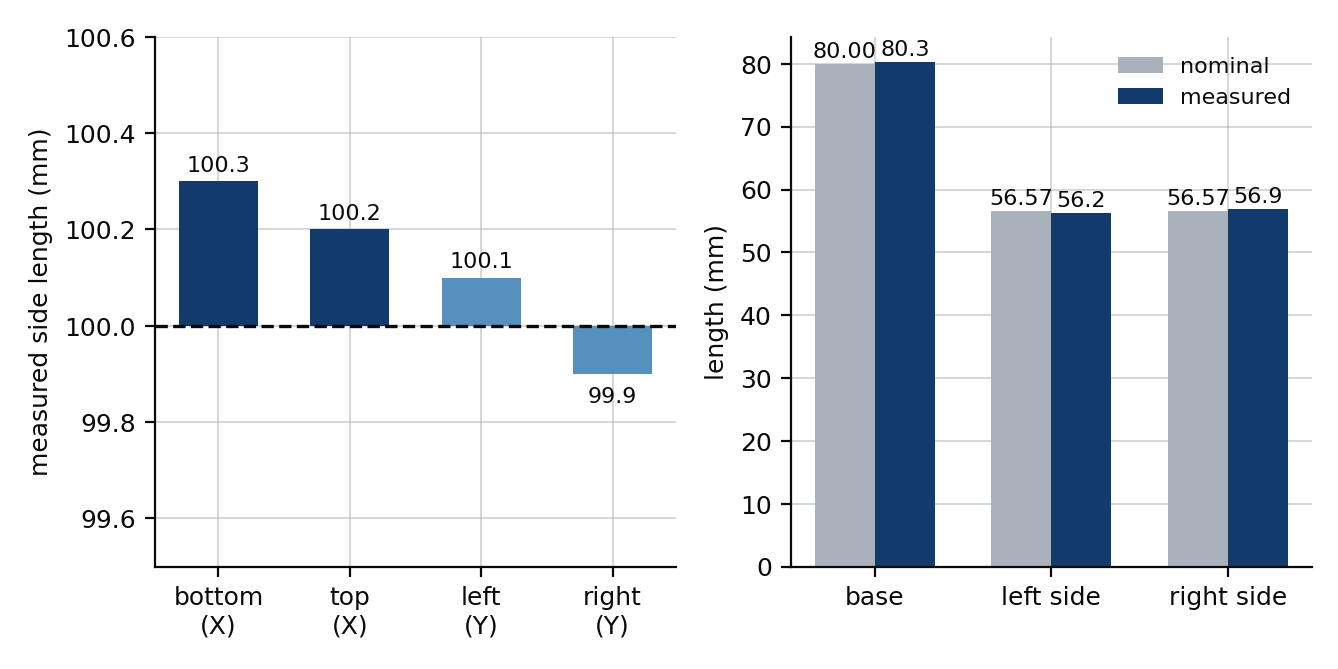
\includegraphics[width=0.95\linewidth]{Figures/res_gantry_geometry.png}
\caption{Measured geometry against nominal. The left panel shows the four sides
of the 100\,mm square, with the dashed line at nominal; the right panel compares
the triangle's measured features with their constructed values.}
\label{fig:res-gantry}
\end{figure}

        Substituting the two sloped sides and the base into
        Equation~\ref{eq:res-shear} gives an apex offset of $d=-0.493$\,mm and a
        squareness error of $\phi=-0.706^{\circ}$. That single value of $d$
        predicts a left sloped side of 56.22\,mm and a right of 56.92\,mm,
        against 56.2\,mm and 56.9\,mm measured, a residual of 0.02\,mm on each.

        \medskip
        \QualificationSection{Observations}

        The worst of the four square sides is 0.30\,mm from nominal and the mean
        absolute error is 0.175\,mm, both inside the 0.5\,mm limit of R5. Both X
        sides are longer than nominal and the two Y sides straddle it.

        The two sloped sides of the triangle differ by 0.70\,mm although they are
        equal by construction. The squareness error solved from them is
        $0.706^{\circ}$. The X scale measured from the square, $+0.250\,\%$,
        predicts a triangle base of 80.20\,mm against 80.30\,mm measured, a
        difference of 0.10\,mm.

        \medskip
        \QualificationSection{Statistical analysis}

        One square and one triangle were measured. That sample supports the
        scale errors and the solved squareness angle, the latter because
        Equation~\ref{eq:res-shear} has one unknown and two measurements and its
        residuals are 0.02\,mm, which is at the resolution of the caliper. It
        does not support a standard deviation, a repeatability figure or a
        tolerance: the 0.40\,mm range across the four sides of the square is the
        spread within one specimen, which combines form error with reading
        error, and is not the variation between repeated draws. Repeated
        specimens are required before a repeatability claim can be made: at
        least five squares and five triangles, with both diagonals of each
        square measured, which would also confirm the squareness angle from a
        second, independent geometry. That measurement is outstanding, and no
        repeatability or tolerance figure is claimed here in its absence.

        What the present sample does support is the one-sided compliance
        statement that R5 asks for. The requirement is an upper bound on
        absolute error, the worst of the four sides is 0.30\,mm, and the
        caliper resolution is 0.01\,mm, so the measured worst case is 0.20\,mm
        clear of the 0.5\,mm limit and the margin is twenty times the reading
        resolution. A repeatability figure would be needed to state a tolerance
        over many draws; it is not needed to report that every side measured on
        this specimen complies.

\medskip
    \QualificationTest{Number of writing styles trained and stored (R6)}

        \medskip
        \QualificationSection{Objectives of the test or experiment}

        To confirm that at least ten writing styles are trained and permanently
        stored, as R6 requires.

        \medskip
        \QualificationSection{Equipment used}

        The stored style profiles and the trained classifier checkpoint on the
        ODROID~N2+ file system.

        \medskip
        \QualificationSection{Test setup and experimental parameters}

        The writer set was reduced from thirteen to eleven during this work:
        writers 151 and 551 were withdrawn and the classifier retrained without
        them. The count below is of the eleven that the deployed system holds.

        \medskip
        \QualificationSection{Steps followed in the test or experiment}

        \begin{enumerate}
        \item List the stored style profiles on the deployed file system.
        \item Read the writer names recorded inside the classifier checkpoint.
        \item Confirm that the two lists agree.
        \end{enumerate}

        \medskip
        \QualificationSection{Results or measurements}

        Eleven writer styles are trained and stored: six from the public
        database, numbered 150, 152, 153, 384, 552 and 588, and five
        photographed for this project, A, B, O, T and Y. The classifier
        checkpoint records the same eleven names, and each writer has a stored
        style profile and a glyph library. All eleven appear in
        Tables~\ref{tab:res-r1-writer} and~\ref{tab:res-r2-writer}.

        \medskip
        \QualificationSection{Observations}

        Eleven styles are stored against a requirement of at least ten. The
        requirement is met with one style in hand.

        \medskip
        \QualificationSection{Statistical analysis}

        Not applicable: the quantity is a count of stored styles, not a
        measurement with error.
